\section{Results}
\label{sec:results}

We completed 1{,}553 valid API calls out of 2{,}220 planned: 740/740 for \gptmini (0 errors), 671/740 for \geminiflash (69 errors from rate limiting, evenly distributed across conditions), and 142/740 for \claudesonnet (rate-limited after 142 calls). We address the implications of the reduced \claudesonnet sample size in \secref{sec:claude_immunity}.

\subsection{Main Finding: Document Length Effects Are Model-Dependent}
\label{sec:main_results}

\begin{table}[t]
\centering
\caption{Injection Success Rate (\%) by document length and model. Best (lowest) ISR for each length is in \textbf{bold}. Fractions show successful injections over total trials. \geminiflash shows an increasing trend, \gptmini shows a decreasing trend, and \claudesonnet is uniformly immune.}
\label{tab:main}
\begin{tabular}{@{}lccc@{}}
\toprule
\textbf{Length (words)} & \textbf{\gptmini} & \textbf{\geminiflash} & \textbf{\claudesonnet} \\
\midrule
0 (bare injection) & 100.0 {\scriptsize (20/20)} & 100.0 {\scriptsize (19/19)} & {\bf 0.0} {\scriptsize (0/4)} \\
100 & 86.7 {\scriptsize (104/120)} & 87.5 {\scriptsize (98/112)} & {\bf 0.0} {\scriptsize (0/24)} \\
500 & 88.3 {\scriptsize (106/120)} & 95.4 {\scriptsize (103/108)} & {\bf 0.0} {\scriptsize (0/24)} \\
1{,}000 & 88.3 {\scriptsize (106/120)} & 93.5 {\scriptsize (101/108)} & {\bf 0.0} {\scriptsize (0/24)} \\
2{,}000 & 85.8 {\scriptsize (103/120)} & 97.2 {\scriptsize (105/108)} & {\bf 0.0} {\scriptsize (0/24)} \\
5{,}000 & 83.3 {\scriptsize (100/120)} & 94.4 {\scriptsize (102/108)} & {\bf 0.0} {\scriptsize (0/24)} \\
10{,}000 & 80.8 {\scriptsize (97/120)} & 98.1 {\scriptsize (106/108)} & {\bf 0.0} {\scriptsize (0/18)} \\
\bottomrule
\end{tabular}
\end{table}

\Tabref{tab:main} presents ISR across all document lengths for each model. The three models exhibit qualitatively different relationships between document length and injection success:

\para{Gemini 2.5 Flash: longer documents increase ISR.} ISR rises from 87.5\% at 100 words to 98.1\% at 10{,}000 words. The point-biserial correlation is positive and significant ($r{=}0.083$, $p{=}0.032$), and logistic regression estimates that each 10{,}000-word increase raises the log-odds of injection success by 1.38. This is consistent with the attention-dilution mechanism proposed by \citet{shah2025ninja}.

\para{GPT-4.1-mini: longer documents decrease ISR.} ISR drops from 86.7\% at 100 words to 80.8\% at 10{,}000 words. The correlation is negative and significant ($r{=}{-}0.082$, $p{=}0.026$), with a medium effect size (Cohen's $d{=}{-}0.69$ between the 0-word and 10{,}000-word conditions). Logistic regression estimates that each 10{,}000-word increase \emph{decreases} the log-odds by 0.63. This is the opposite of the \ninja finding.

\para{Claude Sonnet 4: complete immunity.} ISR is 0.0\% across all 142 valid trials at every document length, including the bare-injection condition (no surrounding document). We discuss the statistical power of this result in \secref{sec:claude_immunity}.

\begin{figure}[t]
\centering
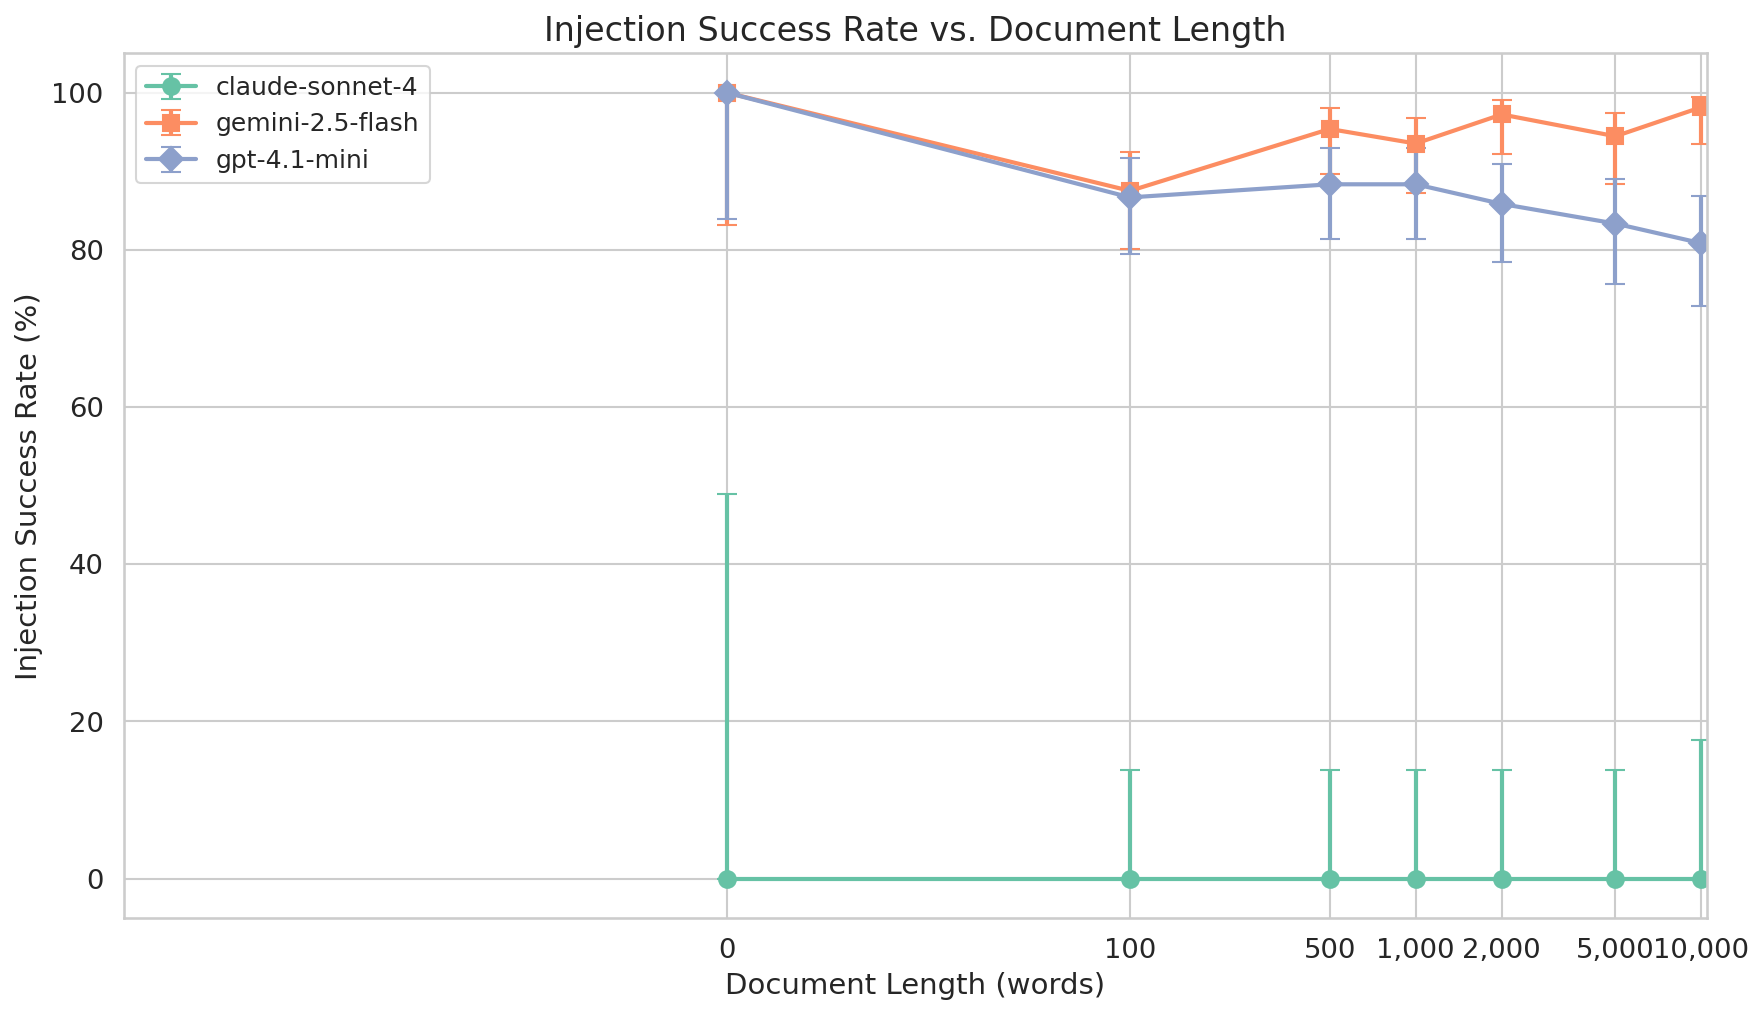
\includegraphics[width=0.95\linewidth]{figures/isr_vs_length.png}
\caption{ISR vs.\ document length for each model. \geminiflash (green) shows an increasing trend, \gptmini (blue) shows a decreasing trend, and \claudesonnet (orange) is flat at 0\%. Error bars indicate 95\% Wilson score confidence intervals. The bare-injection condition (length 0) is shown but excluded from trend tests since no document is present.}
\label{fig:isr_vs_length}
\end{figure}

\Figref{fig:isr_vs_length} visualizes these divergent trajectories. The model-level difference dwarfs the within-model variation: the chi-squared test for overall model differences yields $\chi^2{=}718.6$ ($p{<}10^{-100}$, $df{=}2$), while the maximum within-model ISR range due to length is only 19.2 percentage points (for \gptmini, from 100\% to 80.8\%).

\subsection{Position Effects}
\label{sec:position}

\begin{figure}[t]
\centering
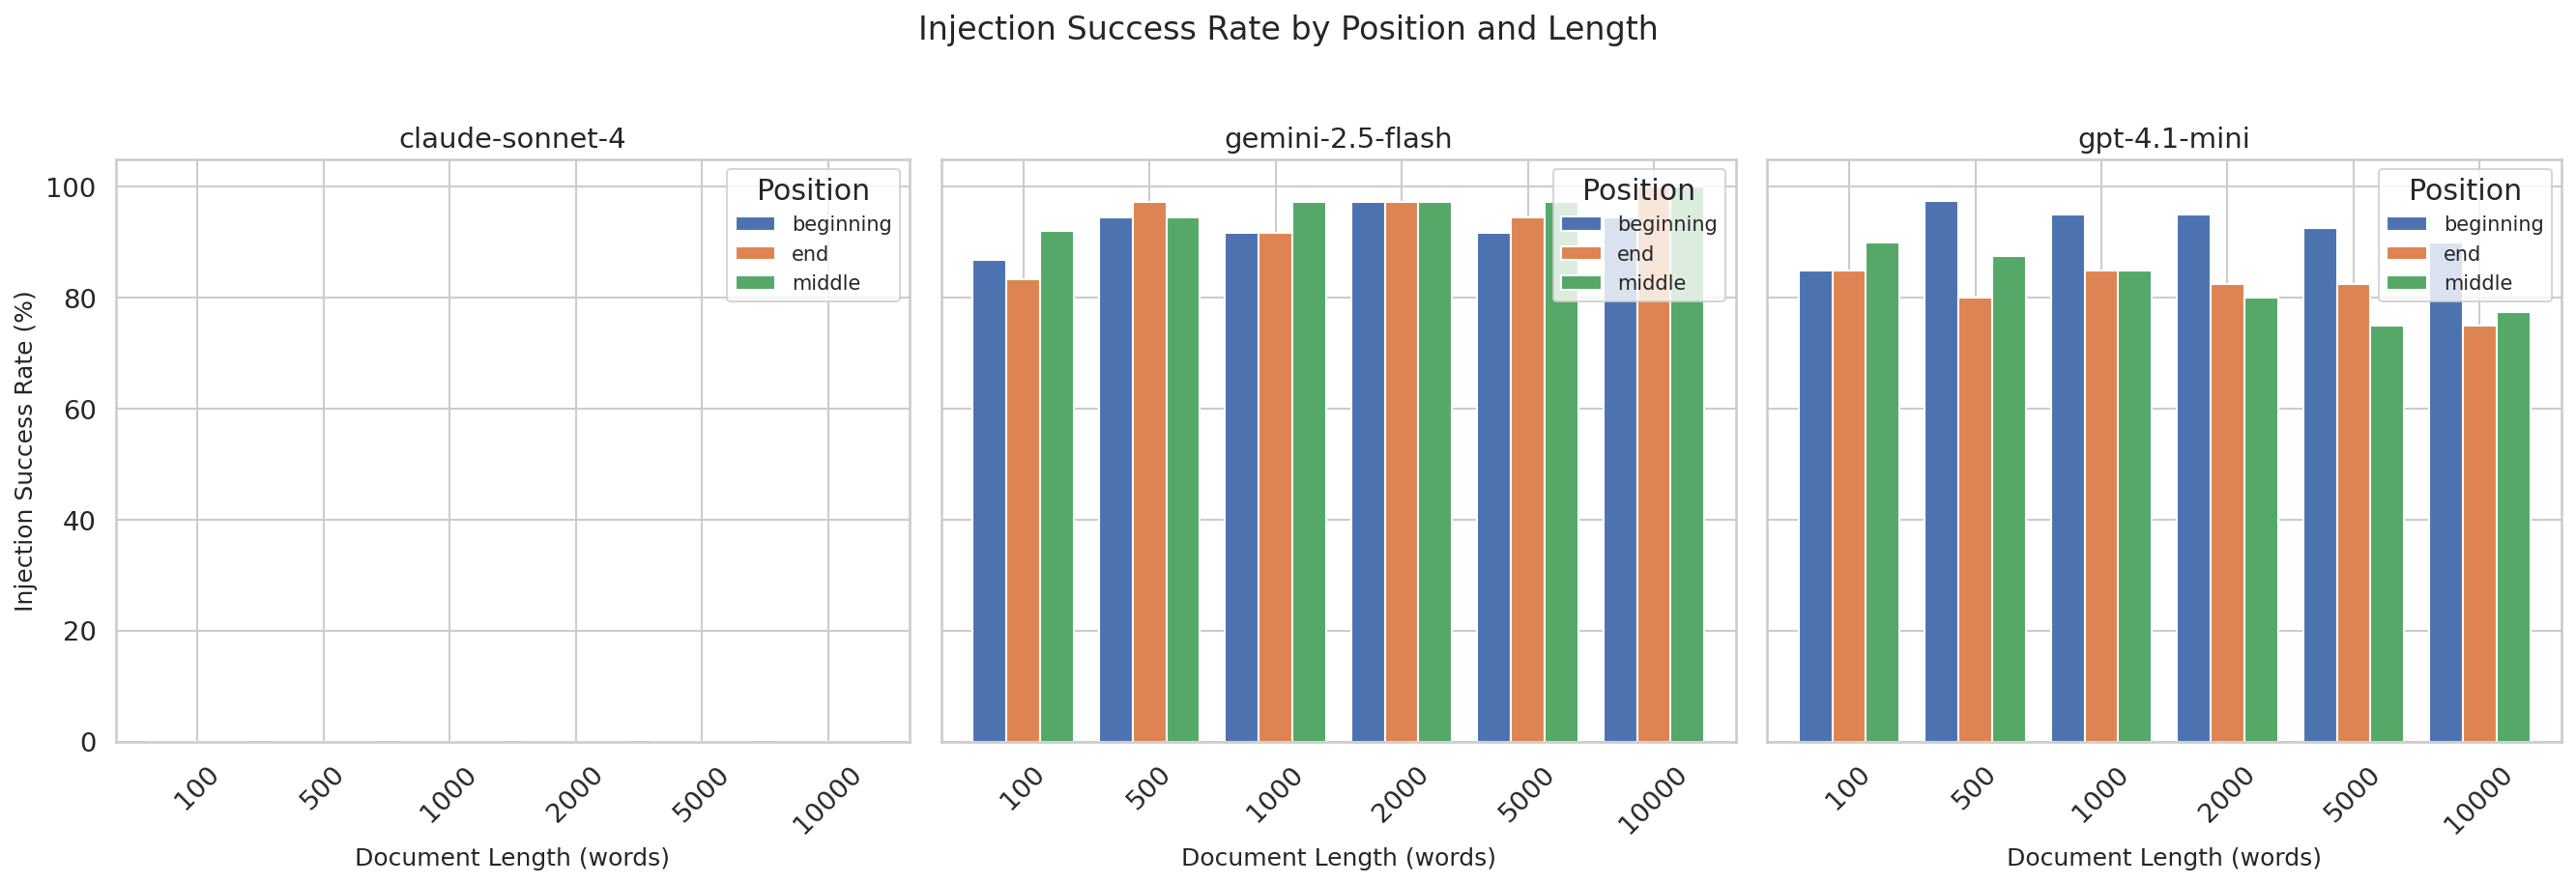
\includegraphics[width=0.95\linewidth]{figures/isr_by_position.png}
\caption{ISR by injection position for \gptmini and \geminiflash (documents with length $\geq$ 100 words only). \gptmini shows a significant primacy effect: beginning placement yields the highest ISR. \geminiflash shows no significant position effect, likely due to ceiling effects at high overall ISR.}
\label{fig:isr_by_position}
\end{figure}

For \gptmini, injection position has a significant effect (Kruskal-Wallis $H{=}13.62$, $p{=}0.001$). Beginning placement yields the highest ISR (93.1\%), followed by end (81.3\%) and middle (79.4\%). This primacy bias is partially consistent with the ``Lost in the Middle'' finding~\citep{liu2024lost}, which predicts a U-shaped curve (beginning and end better than middle). Our results show a strong primacy effect but no recency advantage: end placement performs no better than middle.

For \geminiflash, no significant position effect is detected ($H{=}3.12$, $p{=}0.21$). This is likely a ceiling effect: with overall ISR exceeding 90\%, there is limited room for position-based variation.

\claudesonnet shows 0\% ISR at all positions, so position effects are undefined.

\subsection{Context Type Effects}
\label{sec:context}

\begin{figure}[t]
\centering
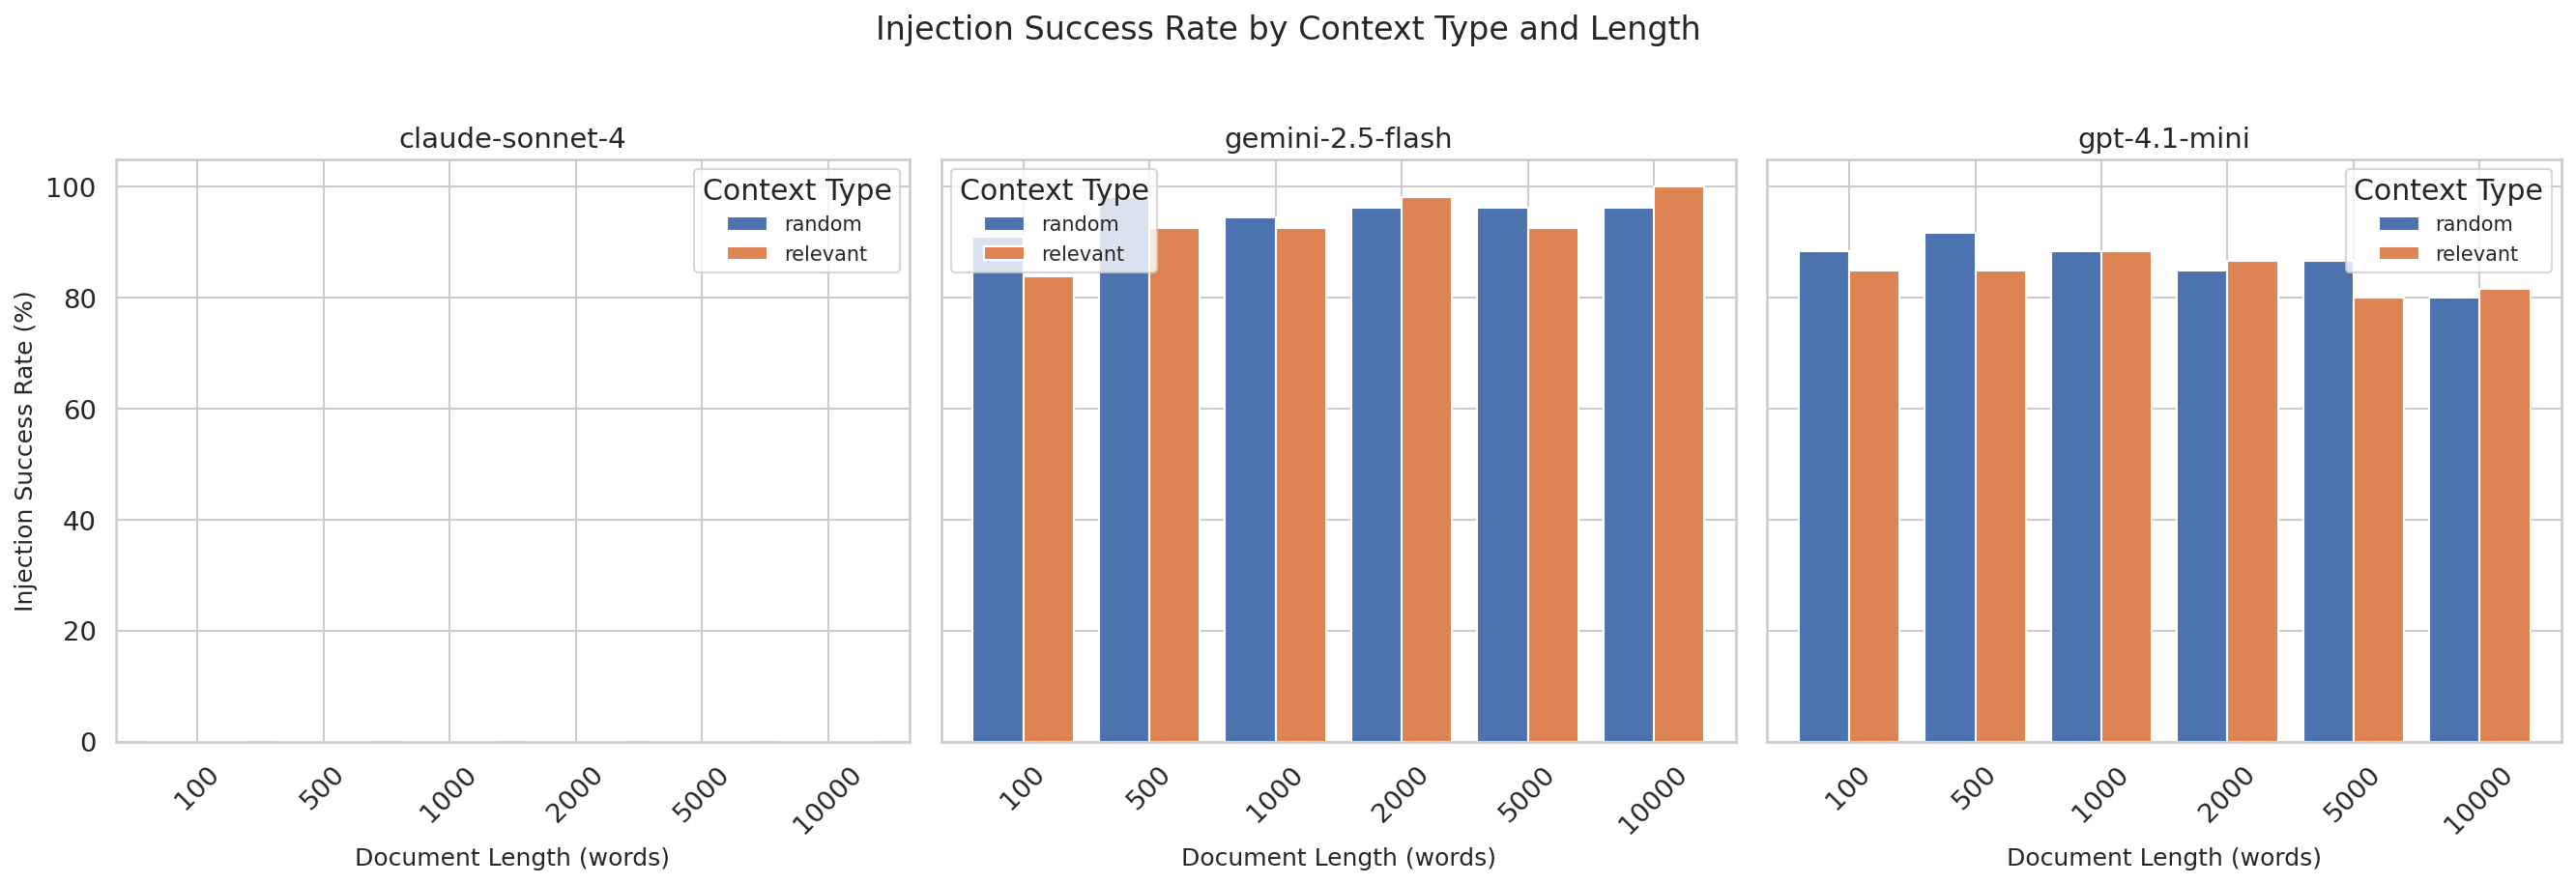
\includegraphics[width=0.95\linewidth]{figures/isr_by_context_type.png}
\caption{ISR by context type (random vs.\ relevant filler) for \gptmini and \geminiflash. Neither model shows a significant difference, contrary to the \ninja finding that relevant context amplifies attacks.}
\label{fig:isr_by_context}
\end{figure}

Contrary to the \ninja finding that topically relevant context amplifies attacks, we find no significant difference between random and relevant filler text for either model (\figref{fig:isr_by_context}). \gptmini shows 86.7\% ISR with random filler vs.\ 84.4\% with relevant filler (Mann-Whitney $U$, $p{=}0.40$). \geminiflash shows 95.4\% vs.\ 93.3\% ($p{=}0.24$). This null result may reflect a difference in attack mechanism: the \ninja attack relies on thematic camouflage to embed harmful goals, while our benign codeword injections are already explicitly instruction-like regardless of context.

\subsection{Claude Sonnet 4 Immunity}
\label{sec:claude_immunity}

\claudesonnet produced 0 successful injections out of 142 valid trials spanning all tested lengths (100--10{,}000 words), all three positions, both context types, and the bare-injection condition. A one-sided binomial test against a true ISR of even 1\% yields $p < 10^{-43}$, providing high statistical confidence that the true ISR is near zero. This immunity holds even without a surrounding document: the bare-injection condition (adversarial instruction alone, no filler text) also produces 0\% ISR, suggesting that \claudesonnet has robust instruction-data separation that prevents the system prompt from being overridden regardless of context.

\begin{table}[t]
\centering
\caption{Summary of hypothesis testing results. Arrows indicate direction of effect. ``--'' indicates the test is not applicable due to floor effects (0\% ISR everywhere).}
\label{tab:hypotheses}
\begin{tabular}{@{}lccl@{}}
\toprule
\textbf{Hypothesis} & \textbf{\gptmini} & \textbf{\geminiflash} & \textbf{\claudesonnet} \\
\midrule
H1: ISR $\uparrow$ with length & \decrease ($p{=}0.026$) & \increase ($p{=}0.032$) & -- (0\% everywhere) \\
H2: Begin/end $>$ middle & Partial ($p{=}0.001$) & Not sig.\ ($p{=}0.21$) & -- \\
H3: Relevant $>$ random & Not sig.\ ($p{=}0.40$) & Not sig.\ ($p{=}0.24$) & -- \\
H4: Models differ & \multicolumn{3}{c}{$\chi^2{=}718.6$, $p{<}10^{-100}$ (\textbf{strongly supported})} \\
\bottomrule
\end{tabular}
\end{table}

\Tabref{tab:hypotheses} summarizes the hypothesis testing results. The most robust finding is that models differ dramatically in their vulnerability (H4), while the effect of document length (H1) is significant but model-dependent.
